\documentclass{standalone}
\usepackage{tikz}
\usetikzlibrary{mindmap}

\begin{document}
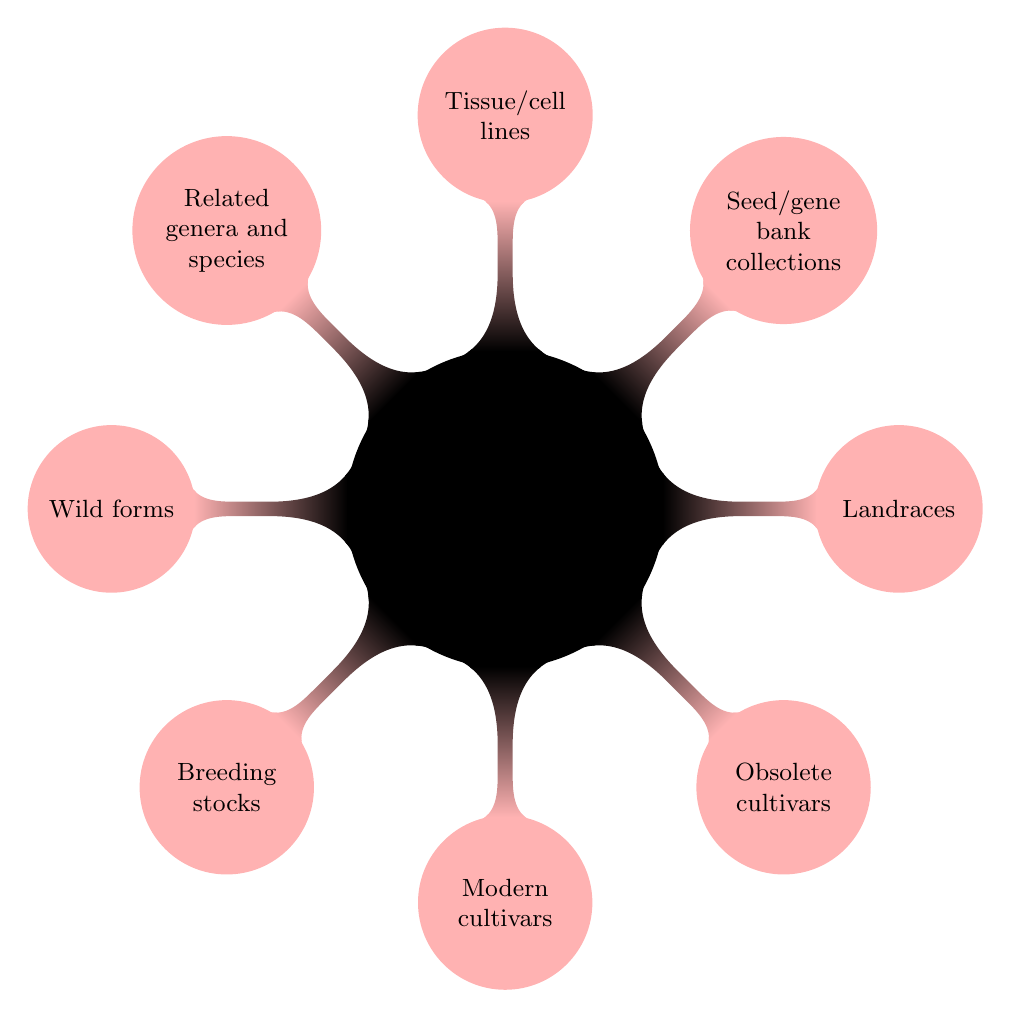
\begin{tikzpicture}[scale=1,mindmap,
                    root concept/.append style={concept color=blue!60,minimum size=1.2cm,inner sep=1pt},
                    level 1 concept/.append style={minimum size=0.8cm,sibling angle=45,inner sep=1pt}]
\node [concept] {Germplasm}
[clockwise from=0]
child[concept color=red!30] {node[concept] {Landraces}}
child[concept color=red!30] {node[concept] {Obsolete cultivars}}
child[concept color=red!30] {node[concept] {Modern cultivars}}
child[concept color=red!30] {node[concept] {Breeding stocks}}
child[concept color=red!30] {node[concept] {Wild forms}}
child[concept color=red!30] {node[concept] {Related genera and species}}
child[concept color=red!30] {node[concept] {Tissue/cell lines}}
child[concept color=red!30] {node[concept] {Seed/gene bank collections}}
;

\end{tikzpicture}
\end{document}